\documentclass[fleqn]{article}
\usepackage{graphicx}

\title{EE214A Design Project}
\author{Jay Smith}
\date{\today}

\begin{document}
\raggedright
\maketitle
\begin{flushleft}

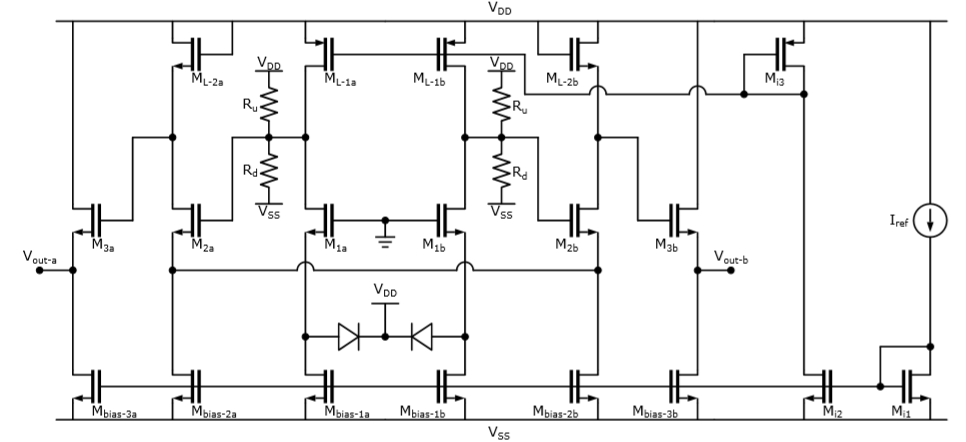
\includegraphics[scale=0.6]{circuit_architecture}

\large{The amplifier under evaluation has 3 stages: 
Common Gate (CG), Common Source (CS), and Common Drain (CD).  In order to analyze, the circuit is broken down into its 3 stages and key parameters are summarized.}\\
\vspace{5mm} 

\begin{tabular}{ | p{6cm} || p{6cm} | }
\hline
Parameter & Spec\\
\hline
Transresistance gain & 42.5k\\
\hline
Output load resistance & 20k\\
\hline
Output load capacitance & 250fF\\
\hline
\end{tabular}
\vspace{10mm}




\newpage
\textbf{Common Gate:}\\
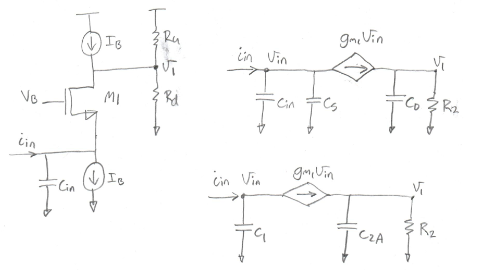
\includegraphics[scale=1.3]{CG_schematic}

\begin{equation}
C_{in} = 100fF
\end{equation}
\begin{equation}
C_S = C_{gs1} + C_{sb1} = cstot (Hspice)
\end{equation}
\begin{equation}
C_D = C_{gd1} + C_{db1} = cdtot (Hspice) \approx 0.58*C_{gs1} = 0.58*(2/3)*(W/L)_1*C_{ox}
\end{equation}
Condensed
\begin{equation}
C_1 = 100fF + C_S
\end{equation}
\begin{equation}
C_{2A} = C_D
\end{equation}

Setting R\textsubscript{u} = R\textsubscript{d} = R
\begin{equation}
R_{L1} = 2*R
\end{equation}

\begin{tabular}{ | p{4cm} || p{4cm} | }
\hline
\multicolumn{2}{ | c | }{ Low Frequency Characteristics }\\
\hline
Transimpedance & R\textsubscript{L1}\\
\hline
Rin & 1/gm1\\
\hline
Rout  & ro\\
\hline
\end{tabular}


\newpage
\textbf{Common Source:}\\
The source of the common source stage is referenced to virtual, small-signal ground in the DM half circuit, so parasitic capacitances to base can be neglected.
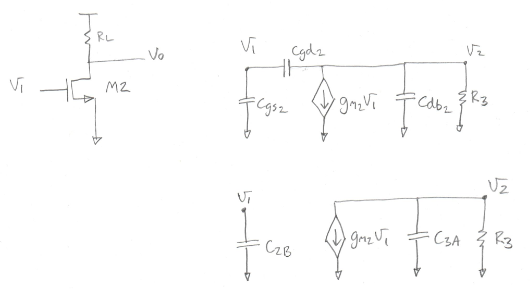
\includegraphics[scale=1.3]{CS_schematic}

Using Miller Approximation:
\begin{equation}
A = g_{m2}*R_{L2}
\end{equation}
\begin{equation}
C_{2B} = C_{gs2} + (1 + A)*C_{gd2}
\end{equation}
\begin{equation}
C_{3A} = C_{db2} + (1 + 1/A)*C_{gd2}
\end{equation}

\begin{tabular}{ | p{4cm} || p{4cm} | }
\hline
\multicolumn{2}{ | c | }{ Low Frequency Characteristics }\\
\hline
Av & -gm2*R\textsubscript{L2}\\
\hline
Rin & inf\\
\hline
Rout  & R\textsubscript{L2}\\
\hline
\end{tabular}

\newpage
\textbf{Common Drain:}
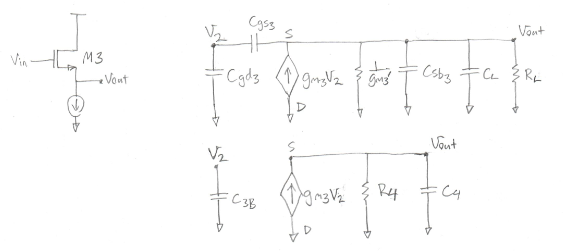
\includegraphics[scale=1.2]{CD_schematic}
\begin{equation}
C_{L} = 250fF
\end{equation}
\begin{equation}
R_{L} = 20k\Omega
\end{equation}
Using Miller Approximation:
\begin{equation}
A \approx -\frac{g_{m3}}{g_{m3}'} \approx -0.84
\end{equation}
\begin{equation}
C_{3B} = C_{gd3} + 0.14*C_{gs3}
\end{equation}
\begin{equation}
C_4 = -0.2*C_{gs3} + C_{sb3} + C_L
\end{equation}
\begin{equation}
R_L = 20k\Omega
\end{equation}

\newpage
\textbf{Full Schematic}
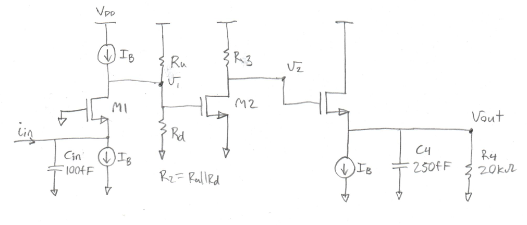
\includegraphics[scale=1]{full_schematic}\\
Low Frequency Transresistance:
\begin{equation}
\frac{v_{out}}{i_{in}} = 0.84*(R_2)*(-g_{m2}*R_3)
\end{equation}
\vspace{5mm}
\textbf{Full Small-Signal Model}
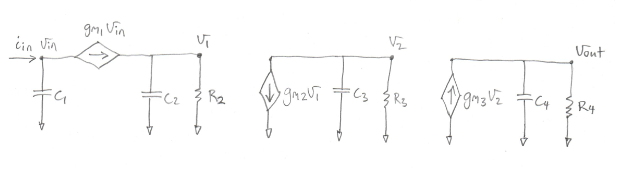
\includegraphics[scale=1]{full_small_signal}
ZVTC bandwidth (conservative approximation)
\begin{equation}
b1 = \frac{1}{g_{m1}}*C_1 + R_2*C_2 + R_3*C_3 + R_4*C_4
\end{equation}
where
\begin{equation}
C_1 = 100fF + cstot1 (Hspice)
\end{equation}
\begin{equation}
R_2 = variable
\end{equation}
\begin{equation}
C_2 = cdtot1 (Hspice) + C_{gs2} + (1 + A)*C_{gd2}
\end{equation}
\begin{equation}
R_3 = variable
\end{equation}
\begin{equation}
C_3 = C_{db2} + (1 + 1/A)*C_{gd2} + C_{gd3} + 0.14*C_{gs3}
\end{equation}
\begin{equation}
R_4 = 20k\Omega
\end{equation}
\begin{equation}
C_4 = -0.2*C_{gs3} + C_{sb3} + 250fF
\end{equation}

\newpage
\textbf{Parameters To Sweep}







\LARGE
APPENDIX\\
\large{The following assumptions are used throughout to simplify analysis.}\\
\begin{tabular}{ | p{3cm} || p{3cm} | }
\hline
\multicolumn{2}{ | c | }{ Simplification of Parasitic Capacitance }\\
\hline
Cdb / Cgs & 0.33\\
\hline
Cgd / Cgs & 0.25\\
\hline
gm / gm'  & 0.84\\
\hline
\end{tabular}

\end{flushleft}
\end{document}